\chapter{Analisis}
\label{chap:analisis}

Pada bab ini akan dijelaskan mengenai analisis pemanfaatan jsoup untuk mengambil data mahasiswa, dan analisis pemanfaatan JavaFX untuk membuat tampilan antarmuka pengguna.

\section{Analisis Pemanfaatan Jsoup}
Untuk mengambil data mahasiswa, diperlukan sumber data mahasiswa tersebut. Sumber data mahasiswa tersebut dapat diperoleh melalui Student Portal UNPAR. Student Portal UNPAR merupakan sebuah situs yang diperuntukkan bagi mahasiswa untuk mendapatkan informasi mengenai profil dan kegiatan akademik mahasiswa tersebut. Mahasiswa dapat mengakses Student Portal UNPAR melalui \textit{URL} \url{https://studentportal.unpar.ac.id/}. Untuk mengakses Student Portal UNPAR, mahasiswa harus melakukan \textit{login} menggunakan \textit{email} dan \textit{password} mahasiswa tersebut.

Aplikasi \textit{screen saver} akan melakukan \textit{http} ke Student Portal UNPAR untuk mendapatkan data untuk setiap kebutuhan dari masing-masing fitur yang ada. Pengambilan data secara langsung dari Student Portal UNPAR dilakukan menggunakan \textit{library} jsoup. Beberapa implementasi pemanfaatan jsoup untuk mengambil data-data tersebut sudah diimplementasikan pada skripsi Andrianto Sugiarto \cite{ifstupor} sebelumnya. Data yang telah didapat dari Student Portal UNPAR kemudian diolah ke dalam SIAModels, dan ditampilkan sesuai dengan fitur-fitur yang ada pada aplikasi Mahasiswa Wali \textit{Screen Saver}.

\subsection{\textit{Login}}
Halaman \textit{Login} (Gambar \ref{fig:3_login} dan \ref{fig:3_login_2}) merupakan halaman dimana mahasiswa memasukkan \textit{email} dan \textit{password} untuk mengakses menu-menu Student Portal UNPAR.

\begin{figure}[H]
	\centering
	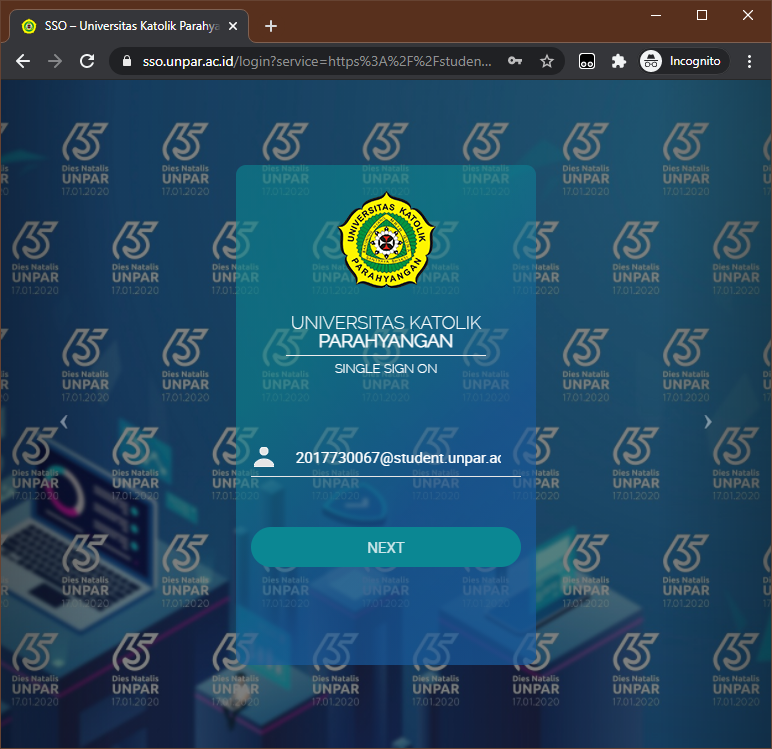
\includegraphics[scale=0.45]{Gambar/login_2.png}
	\caption{Halaman \textit{Login} 1} 
	\label{fig:3_login}
\end{figure}

\begin{figure}[H]
	\centering
	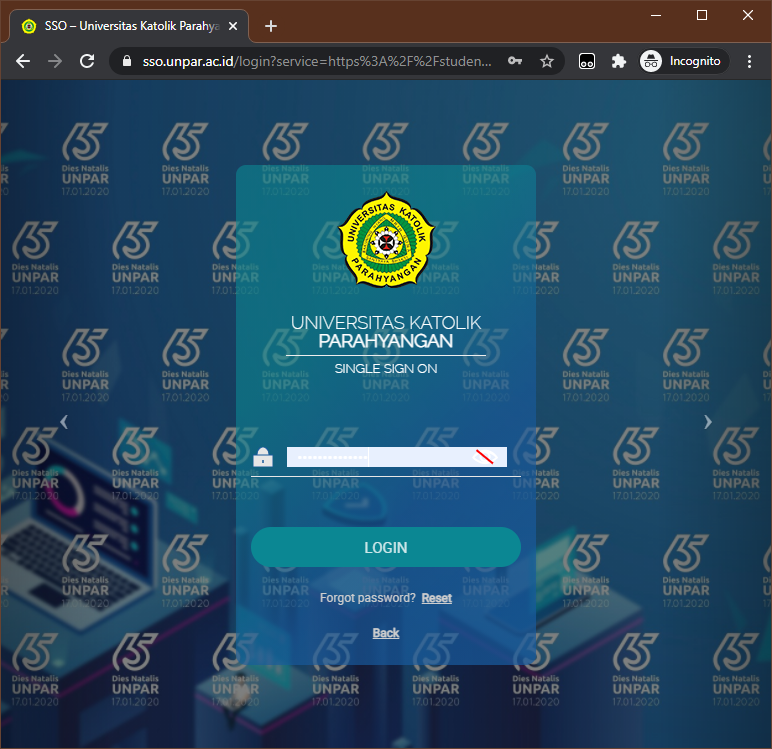
\includegraphics[scale=0.45]{Gambar/login_3.png}
	\caption{Halaman \textit{Login} 2} 
	\label{fig:3_login_2}
\end{figure}

\textit{Login} dilakukan dengan mengirim \textit{request method} POST, dan kemudian mengambil session yang akan digunakan sebagai \textit{cookies} apabila \textit{login} berhasil.
Terdapat beberapa perubahan yang terjadi pada situs Student Portal UNPAR semenjak skripsi Andrianto Sugiarto, yang mengakibatkan perlunya perubahan (Gambar \ref{fig:3_diff_login}) terhadap implementasi jsoup:

\begin{enumerate}
    \item Menyimpan atribut mahasiswa pada kelas tersebut agar tidak perlu melakukan \textit{request} \textit{login} berulang kali ketika mengakses menu-menu Student Portal UNPAR.
    \item Menghapus pemanggilan fungsi validateTLSCertificates() dikarenakan sudah \textit{deprecated} \cite{jsoup}.
    \item Menghapus kueri css "input[name=lt]" dikarenakan kueri tersebut sudah dihapus oleh Student Portal UNPAR.
    \item Menghapus atribut jsessionid dikarenakan tidak dibutuhkan.
\end{enumerate}

\begin{figure}[H]
	\centering
	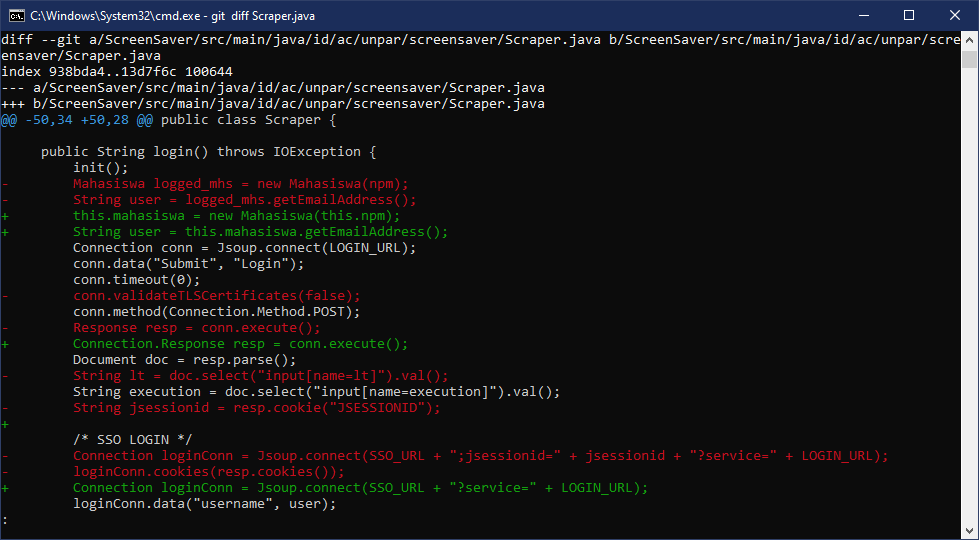
\includegraphics[scale=0.6]{Gambar/diff_login.png}
	\caption{Perubahan Implementasi Jsoup Login} 
	\label{fig:3_diff_login}
\end{figure}

\subsection{Halaman Utama}
Pada Halaman Utama Student Portal UNPAR (Gambar \ref{fig:3_home}), terdapat nama lengkap dan foto dari mahasiswa tersebut yang dapat diambil dan digunakan. Nama mahasiswa dapat diambil dengan melakukan kueri css "div[class=namaUser d-none d-lg-block mr-3]". Foto mahasiswa dapat diambil dengan melakukan kueri css "img[class=img-fluid fotoProfil]".
Terdapat beberapa perubahan (Gambar \ref{fig:3_diff_halaman_utama}) yang perlu dilakukan terhadap skripsi Andrianto Sugiarto:

\begin{figure}[H]
	\centering
	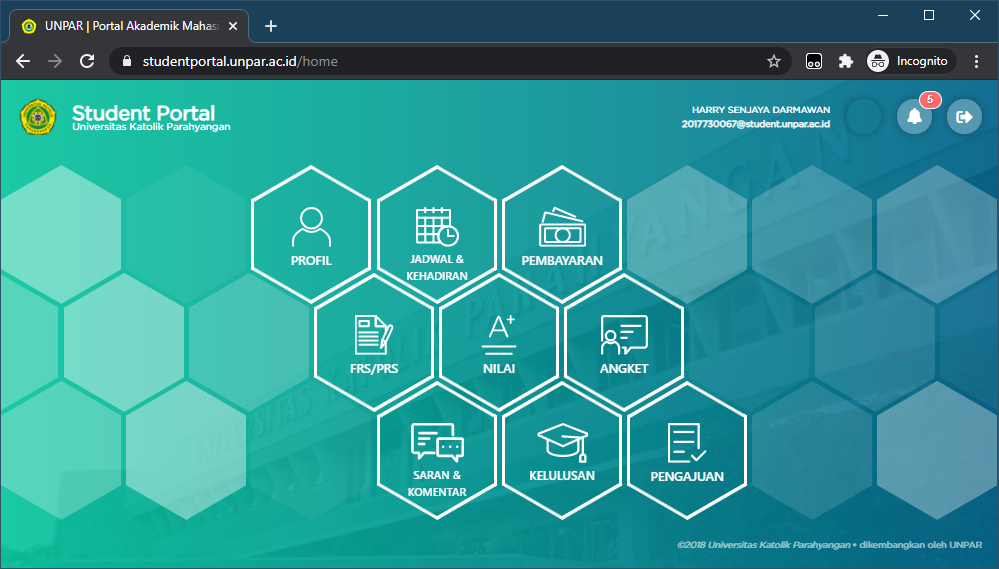
\includegraphics[scale=0.5]{Gambar/home.png}
	\caption{Halaman Utama Student Portal UNPAR} 
	\label{fig:3_home}
\end{figure}

\begin{enumerate}
    \item Menghapus pemanggilan fungsi validateTLSCertificates() dikarenakan sudah \textit{deprecated} \cite{jsoup}.
    \item Menyimpan atribut mahasiswa pada kelas tersebut agar tidak perlu melakukan \textit{request} \textit{login} berulang kali ketika mengakses menu-menu Student Portal UNPAR.
    % \item Sebelumnya semester yang sedang dijalani mahasiswa diambil dari menu FRS/PRS, namun karena terdapat perubahan pada Student Portal UNPAR maka semester yang sedang dijalani mahasiswa diambil dari menu Nilai.
\end{enumerate}

\begin{figure}[H]
	\centering
	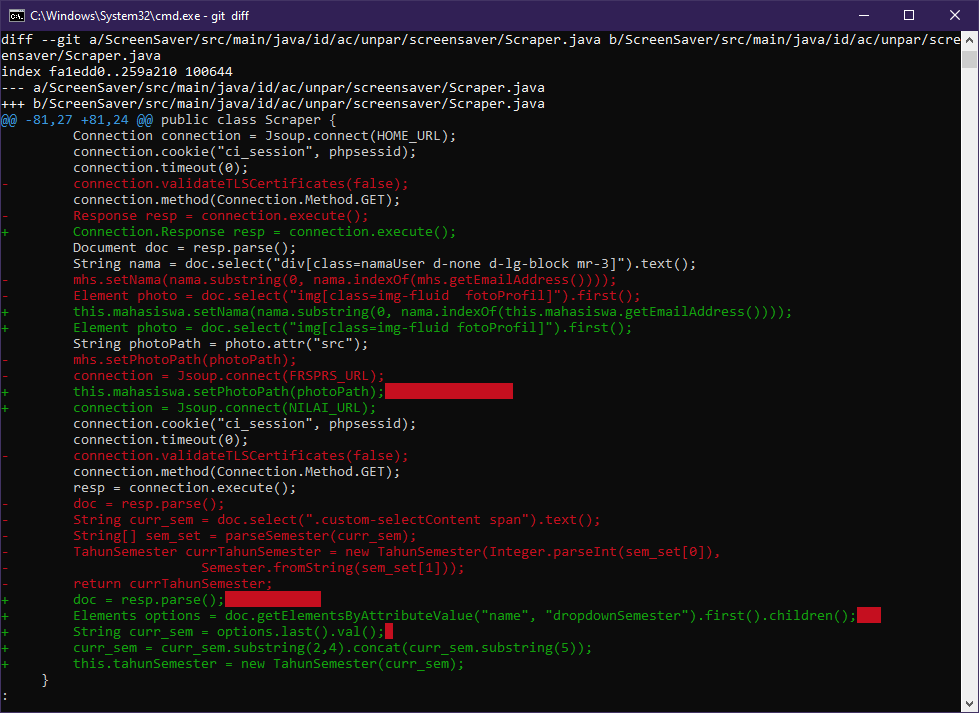
\includegraphics[scale=0.6]{Gambar/diff_requestNamePhotoTahunSemester.png}
	\caption{Perubahan Implementasi Jsoup Halaman Utama} 
	\label{fig:3_diff_halaman_utama}
\end{figure}

Pada halaman utama Student Portal UNPAR juga terdapat beberapa menu yang dapat digunakan sebagai sumber data yaitu:

\subsection{Profil}
    Menu Profil merupakan halaman yang menampilkan data diri mahasiswa (Gambar \ref{fig:3_profil}). Pada halaman ini tempat, dan tanggal lahir mahasiswa akan diambil untuk ditampilkan pada \textit{screen saver}. Implementasi jsoup tersebut belum diimplementasikan pada skripsi Andrianto Sugiarto, sehingga perlu dilakukan penambahan fitur untuk mengambil data tersebut. Tempat, dan tanggal lahir mahasiswa dapat diambil dengan melakukan kueri css "div[class=offset-md-1 col-md-10 col-12 headerWrapper my-0 border-bottom]".
    \begin{figure}[H]
    	\centering
    	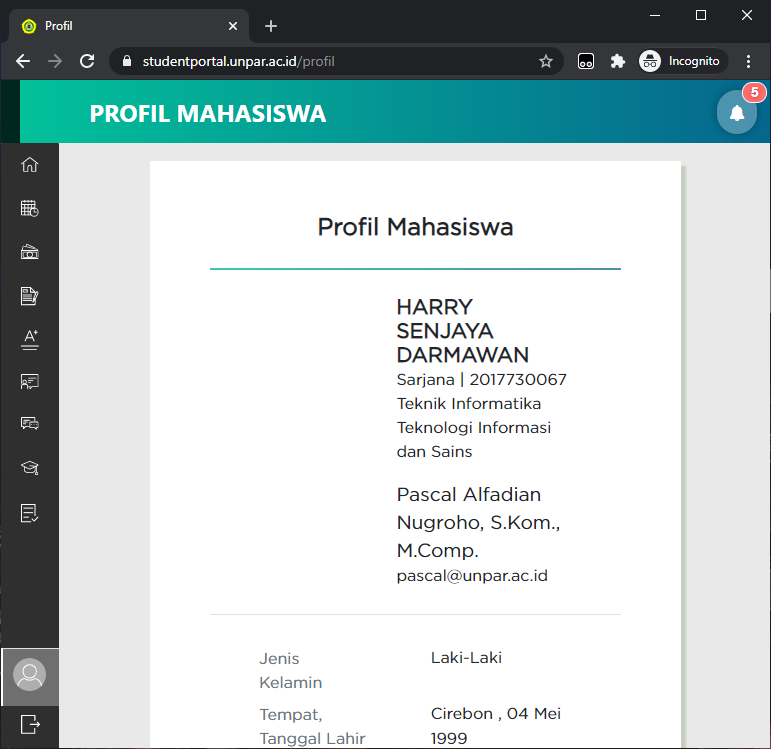
\includegraphics[scale=0.45]{Gambar/profil.png}
    	\caption{Halaman Profil} 
    	\label{fig:3_profil}
    \end{figure}
    
\subsection{Nilai}
    Menu Nilai terdiri dari beberapa submenu:
    
    \begin{itemize}
        \item Nilai per Semester\\
        Submenu ini menampilkan informasi nilai per semester. Mahasiswa dapat melihat nilai sesuai dengan semester yang dipilih (Gambar \ref{fig:3_nilai_per_semester}). 
        % Semester yang sedang diambil oleh mahasiswa dapat digunakan untuk ditampilkan pada \textit{screen saver}. Pengambilan semester tersebut dilakukan dengan mencari elemen dengan nama "dropdownSemester". 
        
        \begin{figure}[H]
        	\centering
        	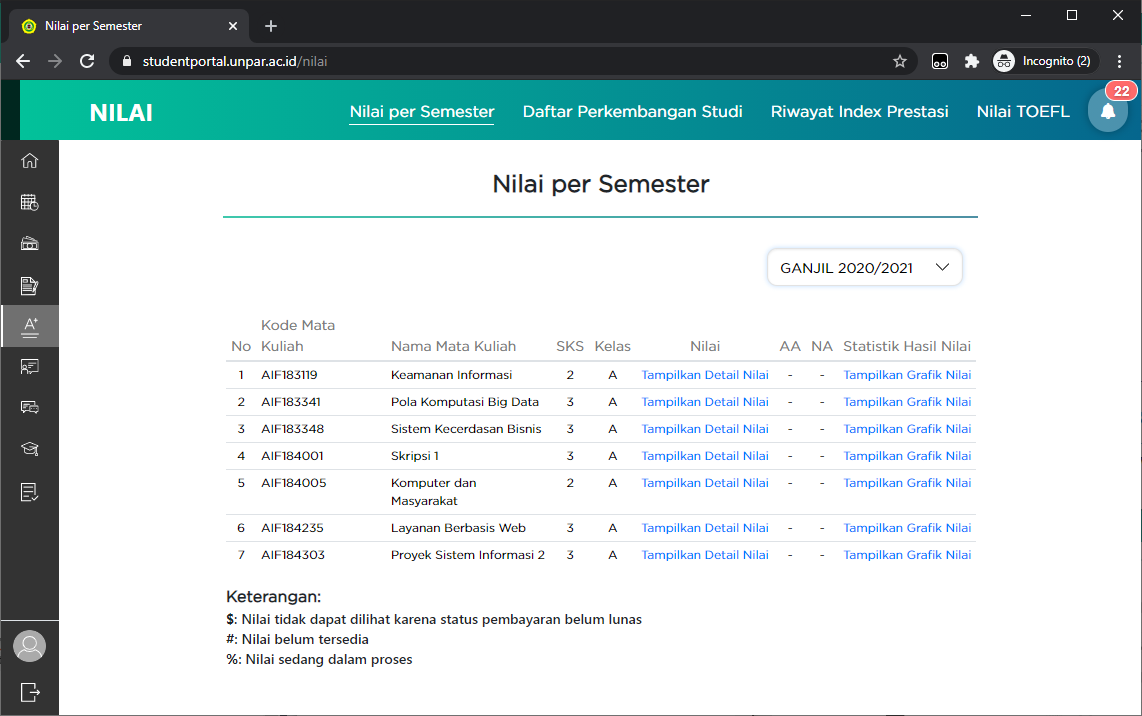
\includegraphics[scale=0.4]{Gambar/nilai_per_semester.png}
        	\caption{Halaman Nilai Per Semester} 
        	\label{fig:3_nilai_per_semester}
        \end{figure}
        
        \item Daftar Perkembangan Studi\\
        Submenu ini menampilkan seluruh riwayat mata kuliah dan nilai yang pernah ditempuh mahasiswa (Gambar \ref{fig:3_dps_1}). Submenu ini juga menampilkan statistik sks, nilai, dan indeks prestasi mahasiswa (Gambar \ref{fig:3_dps_2}).
        \begin{figure}[H]
        	\centering
        	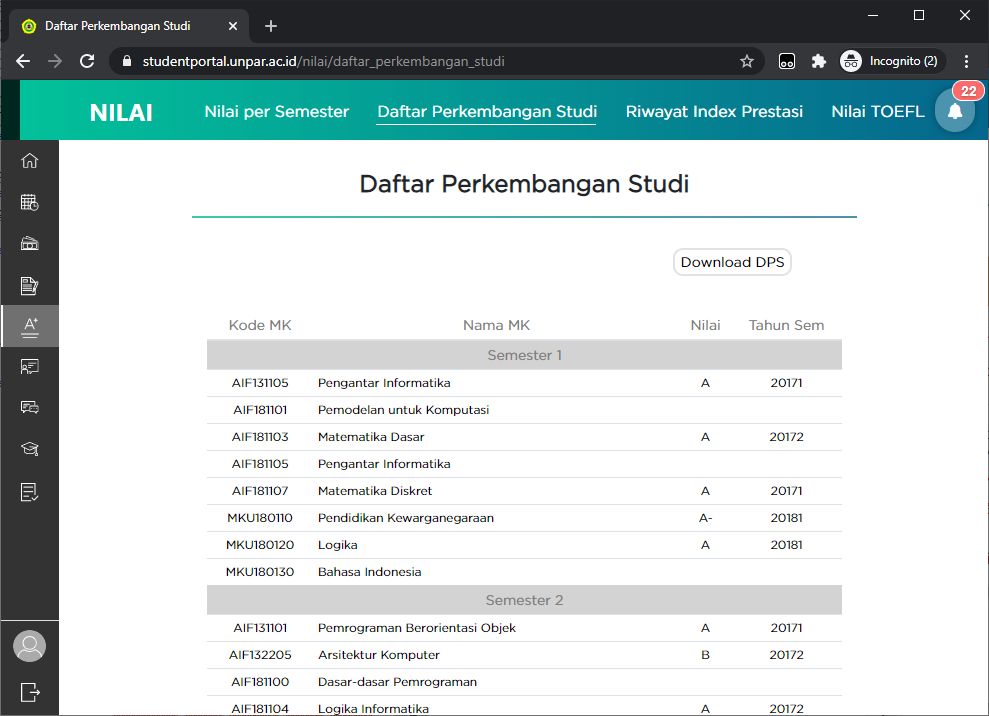
\includegraphics[scale=0.4]{Gambar/nilai_dps_1.png}
        	\caption{Halaman Daftar Perkembangan Studi (1)} 
        	\label{fig:3_dps_1}
        \end{figure}
        
         \begin{figure}[H]
        	\centering
        	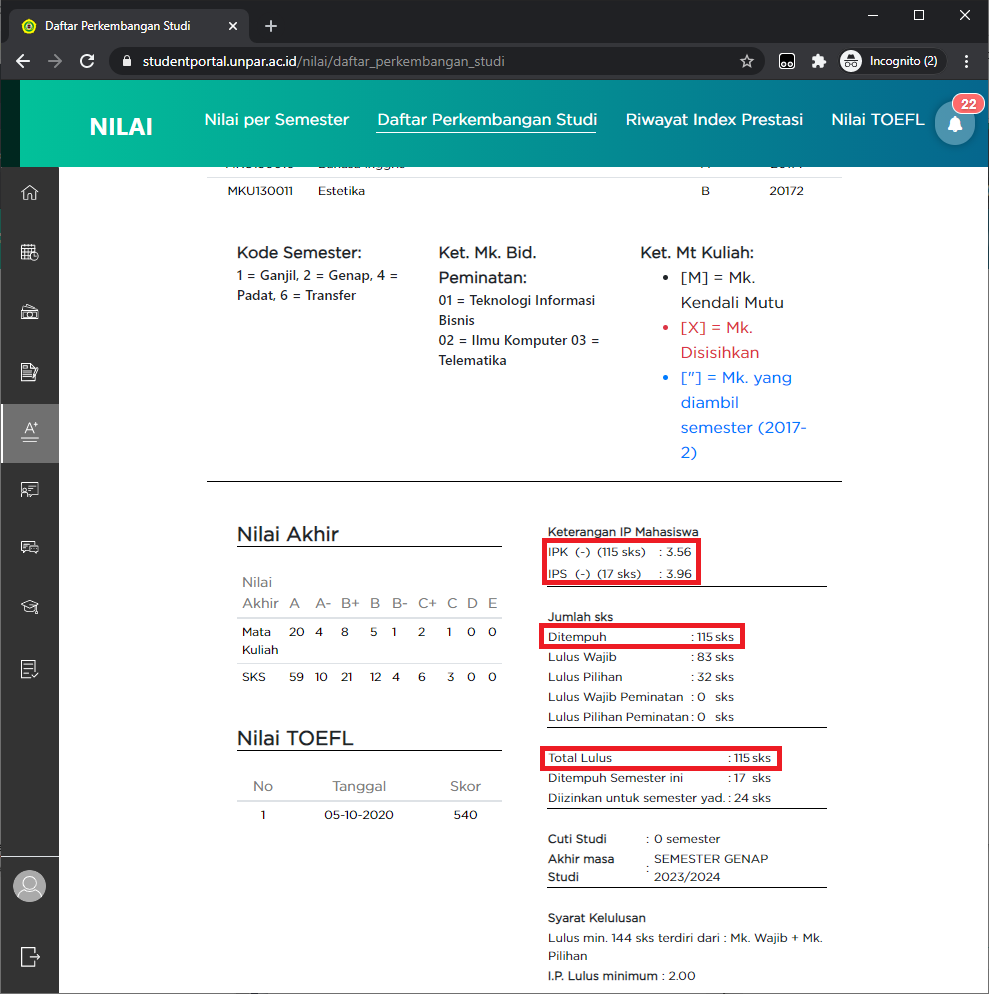
\includegraphics[scale=0.4]{Gambar/nilai_dps_2.png}
        	\caption{Halaman Daftar Perkembangan Studi (2)} 
        	\label{fig:3_dps_2}
        \end{figure}
        Data yang dapat dimanfaatkan dari halaman ini adalah IPK, IPS, jumlah sks yang lulus, dan jumlah sks yang ditempuh. Namun, pada SIAModels sudah terdapat \textit{method} yang melakukan kalkulasi untuk mendapatkan data-data tersebut, sehingga tidak perlu dilakukan pengambilan data menggunakan jsoup. Untuk dapat memanfaatkan \textit{method} tersebut diperlukan seluruh riwayat mata kuliah dan nilai yang pernah ditempuh mahasiswa, sehingga perlu dilakukan pengambilan data menggunakan jsoup.  Implementasi pengambilan data tersebut sudah diimplementasikan sebelumnya pada skripsi Andrianto Sugiarto. Proses dari pengambilan data tersebut yaitu:
        \begin{itemize}
            \item Mengambil data nilai berdasarkan tahun dan semester dengan melakukan kueri css menggunakan kueri ``select\#dropdownSemester.custom-select.mr-3''.
            \item Dikarenakan perlunya melakukan koneksi berkali-kali sebanyak semester yang telah ditempuh mahasiswa, sehingga dibutuhkan waktu yang tidak sebentar. Karena pada halaman nilai tidak dapat menampilkan seluruh semester seperti Student Portal yang lama, sehingga untuk mengatasi masalah ini dibuat menjadi paralel. Untuk itu dibuat kelas yang mengimplementasikan kelas \textit{interface} \texttt{Runnable}, yaitu kelas \texttt{MultipleRequest}. Kelas inilah yang melakukan koneksi ke setiap semester yang telah ditempuh mahasiswa, dan mengambil data-data tersebut.
        \end{itemize}
        Namun, terdapat beberapa perubahan (Gambar \ref{fig:3_diff_halaman_dps}) yang perlu dilakukan:
        \begin{enumerate}
            \item Menghapus pemanggilan fungsi validateTLSCertificates() dikarenakan sudah \textit{deprecated} \cite{jsoup}.
            \item Indeks yang digunakan untuk melakukan keri css berubah, sehingga untuk mengantisipasi tersebut, indeks yang digunakan menjadi \textit{size} dari kueri css dikurangi 1.
        \end{enumerate}
        \begin{figure}[H]
        	\centering
        	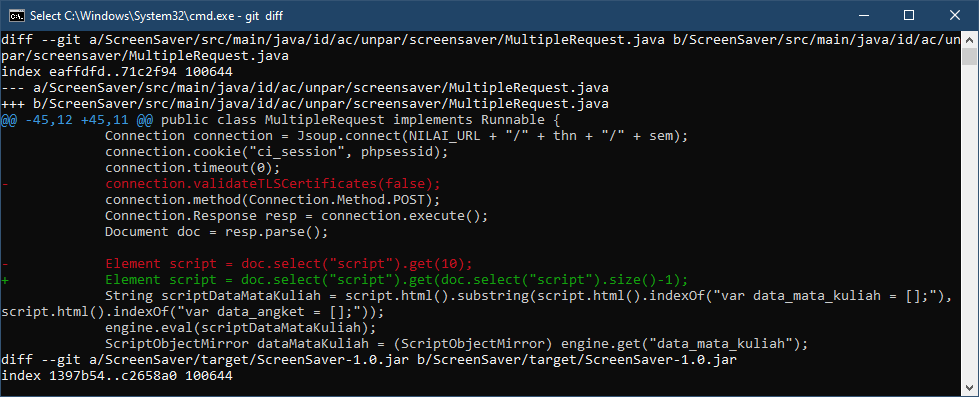
\includegraphics[scale=0.4]{Gambar/diff_multipleRequest.png}
        	\caption{Perubahan Implementasi Jsoup Halaman Daftar Perkembangan Studi} 
        	\label{fig:3_diff_halaman_dps}
        \end{figure}
        
        \item Riwayat Indeks Prestasi\\
       Submenu ini menampilkan seluruh riwayat Indeks Prestasi Semester (IPS) dan Indeks Prestasi Kumulatif (IPK) setiap semester mahasiswa (Gambar \ref{fig:3_rip}).
       
       \begin{figure}[H]
        	\centering
        	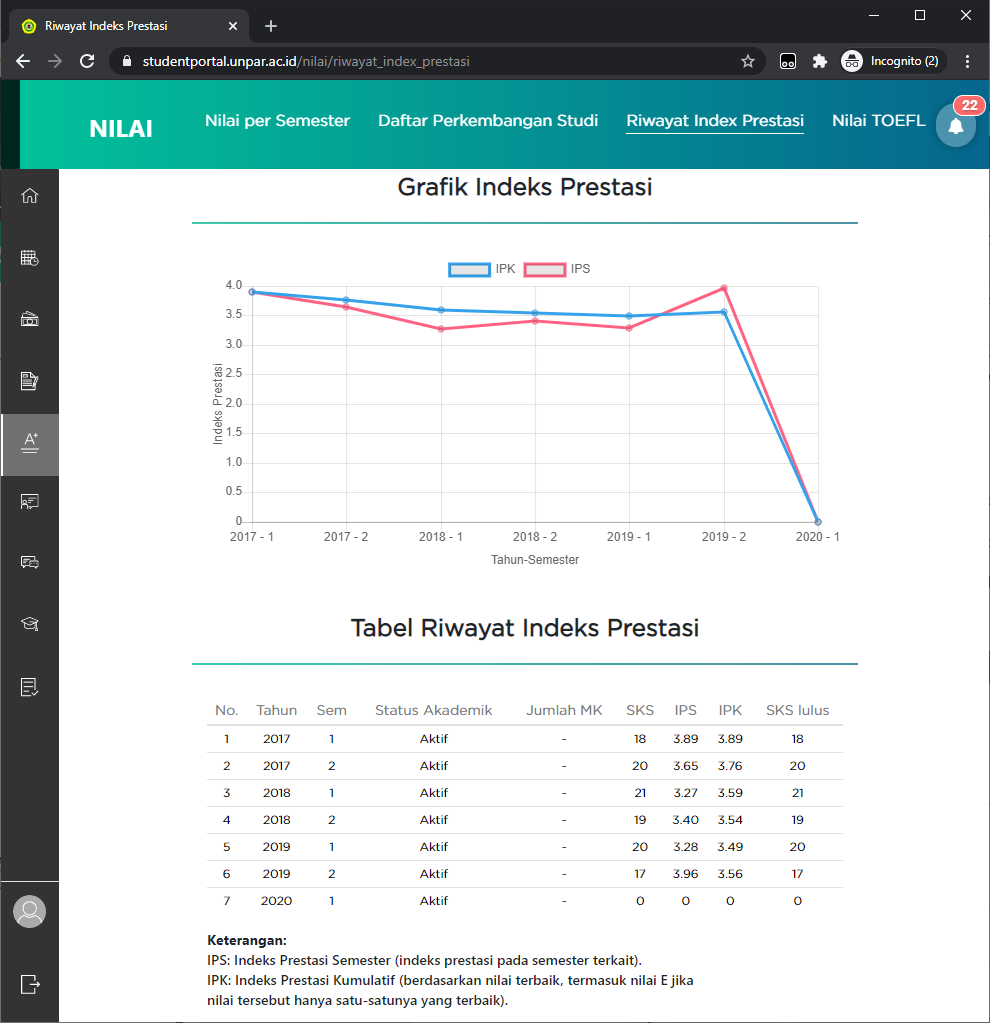
\includegraphics[scale=0.4]{Gambar/nilai_rip.png}
        	\caption{Halaman Riwayat Indeks Prestasi} 
        	\label{fig:3_rip}
        \end{figure}
        
        \item Nilai TOEFL\\
       Submenu ini menampilkan seluruh riwayat skor dan detail skor \textit{Test of English as Foreign Language} (TOEFL) yang pernah ditempuh mahasiswa (Gambar \ref{fig:3_toefl}). Riwayat skor tersebut dapat diambil dengan melakukan kueri css menggunakan kueri “table”, “tbody”, dan “tr”.
       Terdapat beberapa perubahan yang terjadi pada halaman TOEFL semenjak skripsi Andrianto Sugiarto, yang mengakibatkan perlunya perubahan (Gambar \ref{fig:3_diff_toefl}) terhadap implementasi jsoup:

        \begin{enumerate}
            \item Menyimpan atribut mahasiswa pada kelas tersebut agar tidak perlu melakukan \textit{request} \textit{login} berulang kali ketika mengakses menu-menu Student Portal UNPAR.
            \item Menghapus pemanggilan fungsi validateTLSCertificates() dikarenakan sudah \textit{deprecated} \cite{jsoup}.
            \item Perubahan format tanggal TOEFL pada Student Portal UNPAR menjadi dd-mm-yyyy.
        \end{enumerate}
       
       \begin{figure}[H]
        	\centering
        	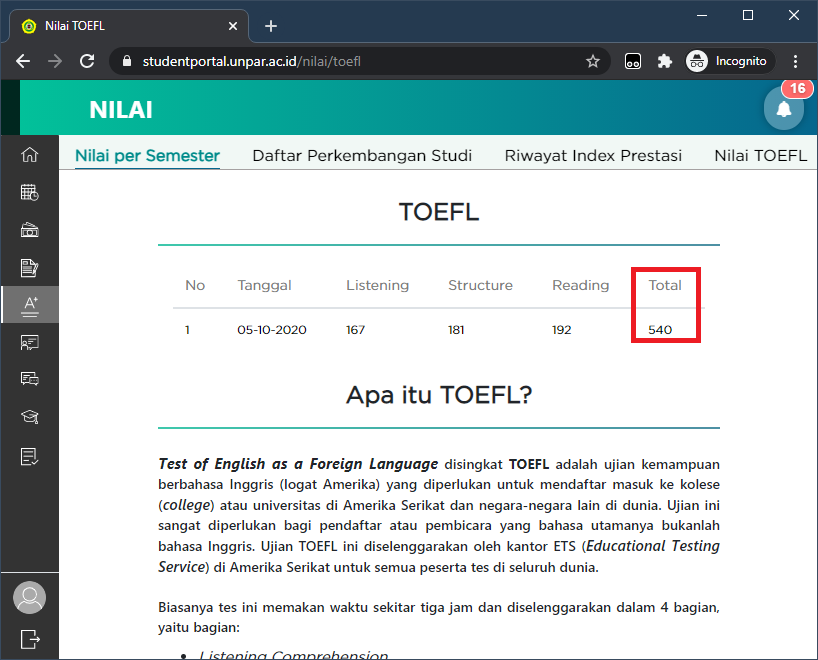
\includegraphics[scale=0.45]{Gambar/nilai_toefl.png}
        	\caption{Halaman Nilai TOEFL} 
        	\label{fig:3_toefl}
        \end{figure}
        
        \begin{figure}[H]
        	\centering
        	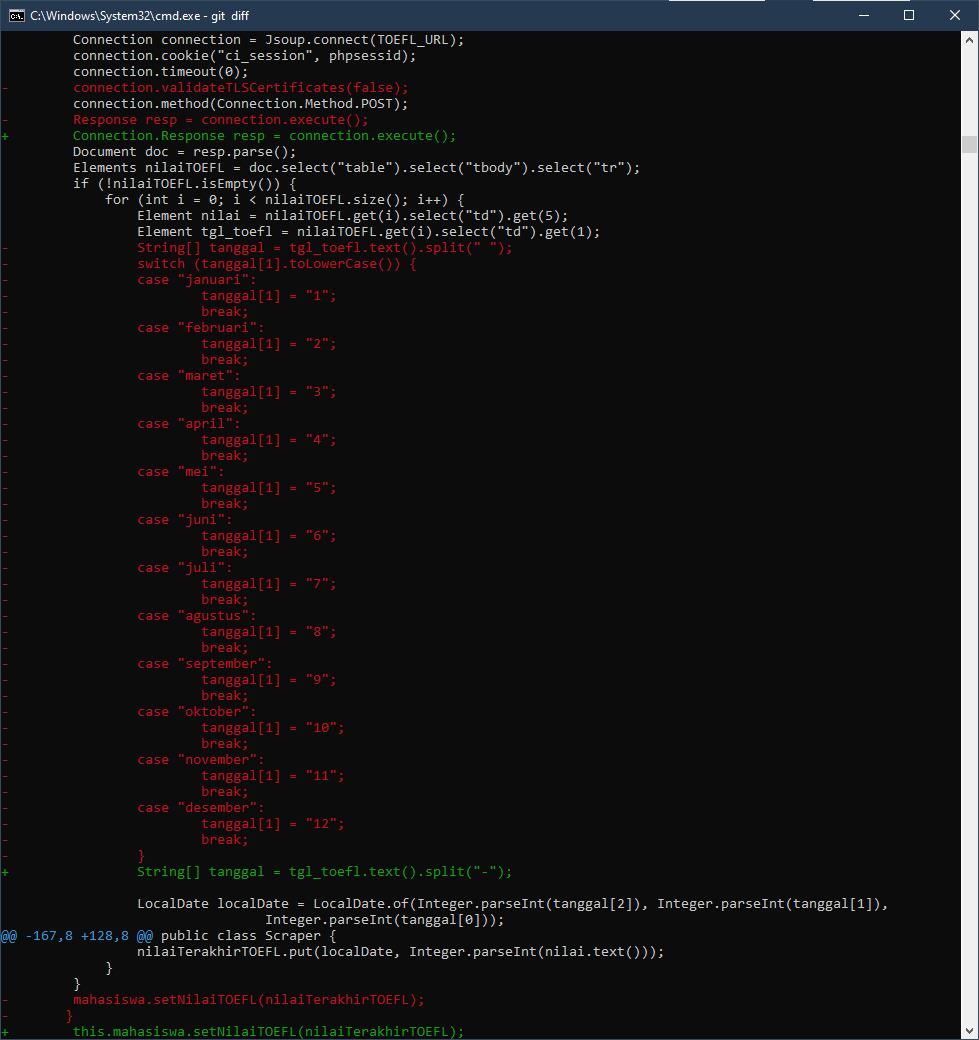
\includegraphics[scale=0.52]{Gambar/diff_toefl.png}
        	\caption{Perubahan Implementasi Jsoup TOEFL} 
        	\label{fig:3_diff_toefl}
        \end{figure}
        
        
    \end{itemize}


